\documentclass[10pt,t]{beamer}

\usetheme[progressbar=frametitle,sectionpage=none]{metropolis}

\usepackage{booktabs}
\usepackage[scale=2]{ccicons}

\usepackage{pgfplots}
\usepgfplotslibrary{dateplot}

\usepackage{xspace}
\newcommand{\themename}{\textbf{\textsc{metropolis}}\xspace}

\usepackage{tikz}
\usetikzlibrary{shapes.geometric, arrows}
\tikzset{font=\scriptsize}
\tikzstyle{startstop} = [rectangle, rounded corners, minimum width=2.7cm,%
minimum height=0.6cm, text centered, draw=black, fill=mLightBrown!50]
\tikzstyle{compute} = [rectangle, minimum width = 2.7cm, minimum height = 0.7cm,%
text centered, draw=black, fill=mLightGreen!40]
\tikzstyle{logic} = [diamond, minimum width = 1.2cm,%
text centered, draw=black, fill=mDarkTeal, text=white]
\tikzstyle{data} = [circle, minimum width=0.5cm,text centered,%
draw=black,fill=white]
\tikzstyle{arrow} = [thick,->,>=stealth]
\tikzstyle{line} = [thick]

%% symbols
\newcommand{\bX}{\mathbf{X}}
\newcommand{\bY}{\mathbf{Y}}
\newcommand{\mat}[1]{\mathbf{#1}}
\renewcommand{\vec}[1]{\boldsymbol{#1}}

\title{Predicting bus arrival using ``imaginary buses''}
\date{June 22, 2016}
\author{Tom Elliott}
\institute{Supervised by Professor Thomas Lumley\\[2em]

\includegraphics[height=1.5cm]{stat-logo.png}}
%Department of Statistics\\University of Auckland}

%\titlegraphic{\hfill
\includegraphics[height=1.5cm]{stat-logo.png}}

\begin{document}

\maketitle



\begin{frame}{Bus Arrival Time Prediction}
  
  \textbf{Goal:} 
  \alert<2>{to predict the} arrival time of buses at \alert<2>{future} stops as accurately as possible,
  and communicate the remaining uncertainty to commuters.

  \onslide<3->
  \vspace{1cm}
  \textbf{Proposed solution:} particle filter
  \begin{itemize}
  \item<4-> \textbf{particle}: an ``imaginary bus'', a plausible trajectory for the real bus
  \item<5-> \textbf{filter}: only keep imaginary buses that are likely given updated position
  \end{itemize}

\end{frame}


% \begin{frame}{Bus arrival time prediction}
%   The problem: \emph{predicting future arrival times of buses} \ldots
%   \onslide<2-> accurately!

  
%   \vspace{1cm}
%   \onslide<3->
%   Our solution:
%   \begin{itemize}
%   \item<alert@4> particle filter
%   \item prediction intervals
%   \item real-time speed information
%   \end{itemize}

% \end{frame}


\begin{frame}{Particle Filter}
  
  Instead of dealing with a \alert<1>{distribution} and \alert<1>{estimating the parameters}\\
  e.g. $\theta \sim \mathcal{N}(\mu, \sigma^2)$

  \begin{overprint}
    \onslide<1>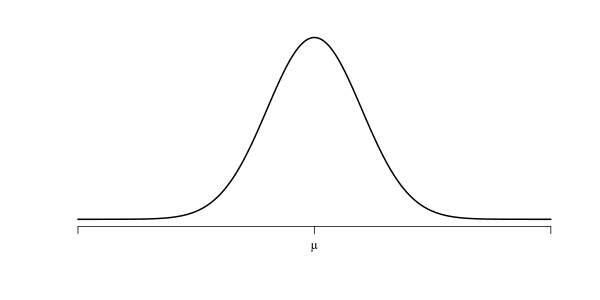
\includegraphics[width=10cm]{normal_dist.png}
    \onslide<2->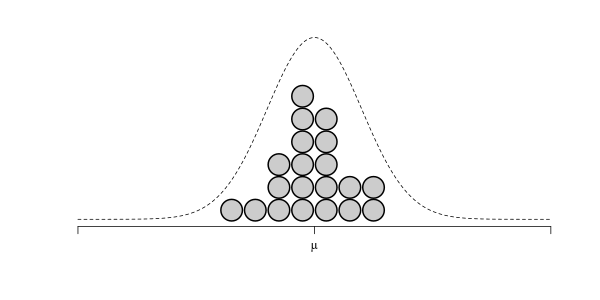
\includegraphics[width=10cm]{particle_dist.png}
  \end{overprint}
  
  \pause
  A particle filter uses ``particles'' that \alert<2>{approximate the distribution}.
  
  \pause
  \textbf{Advantage:} model \alert<3>{dynamics} of each \alert<3>{individual particle} separately.
  
\end{frame}


\begin{frame}{Simple Example of Particle Filter}

  A bus driving down a one dimensional road.
  \onslide<+->

  \begin{itemize}[<+- | alert@+>]
  \item Start with an imaginary fleet
  \item Let each bus drive along the road and end up somewhere
  %\item Add some noise \ldots 
  \item Ask real bus where it (thinks it) actually is
  \item Weight imaginary buses by distance to the real one
  \item Filter imaginary fleet based on weights
  \end{itemize}
  
  \begin{overprint}
    \onslide<2>
    \centering
    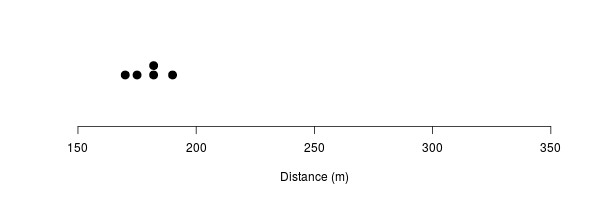
\includegraphics[width=0.8\textwidth]{figs/pf1-frame1.png}
    %\onslide<3>
    %\centering
    %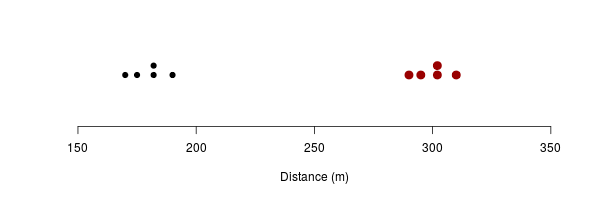
\includegraphics[width=0.8\textwidth]{figs/pf1-frame2.png}
    \onslide<3>
    \centering
    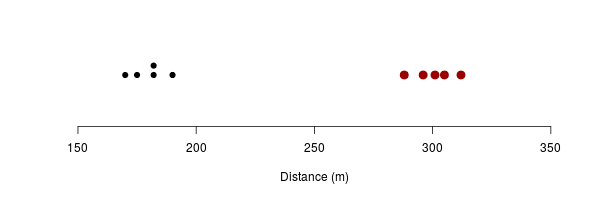
\includegraphics[width=0.8\textwidth]{figs/pf1-frame3.png}
    \onslide<4>
    \centering
    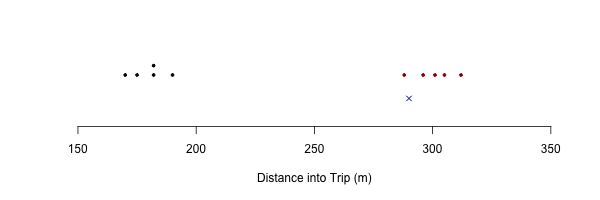
\includegraphics[width=0.8\textwidth]{figs/pf1-frame4.png}
    \onslide<5>
    \centering
    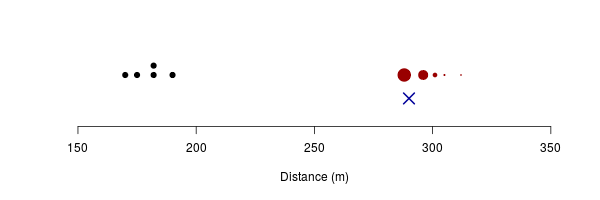
\includegraphics[width=0.8\textwidth]{figs/pf1-frame5.png}
    \onslide<6->
    \centering
    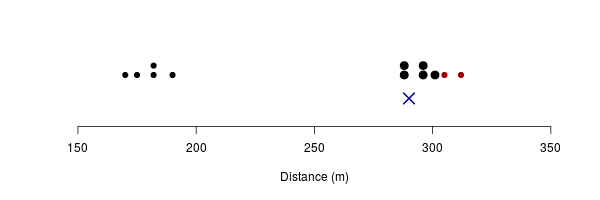
\includegraphics[width=0.8\textwidth]{figs/pf1-frame6.png}
  \end{overprint}

  \onslide<+->
\end{frame}


\begin{frame}{Real Example}
  Buses travel fixed routes, so think of distance along a 2-dimensional line.
  
  \onslide<2->
  Route 049, Henderson -- Britomart:
  
  {\centering
  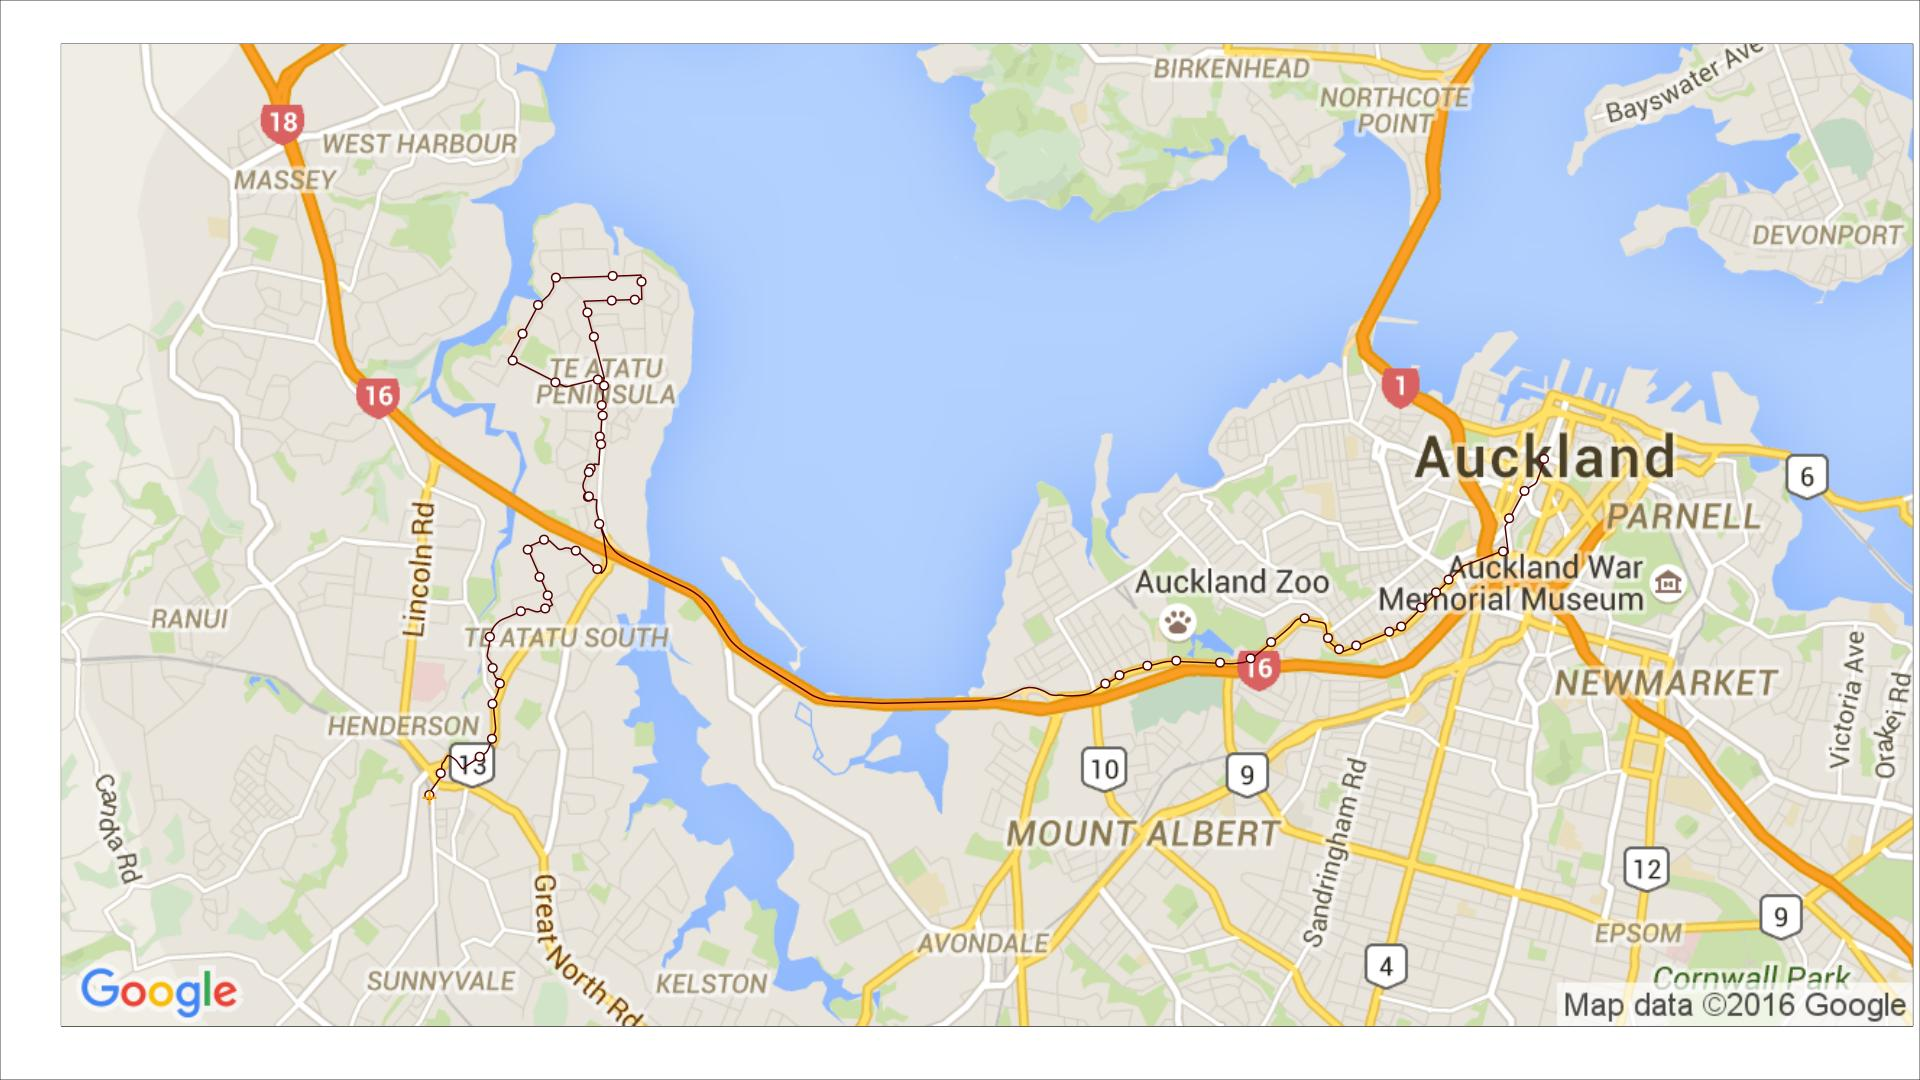
\includegraphics[width=\textwidth]{pf/particle_map001.jpg}}

  \footnotesize\url{https://www.stat.auckland.ac.nz/~tell029/phd/animations/route049.gif}
\end{frame}

{ % all template changes are local to this group.
    \setbeamercolor{background canvas}{bg=white}
    \begin{frame}[plain]
        \begin{tikzpicture}[remember picture,overlay]
            \node[at=(current page.center)] {
                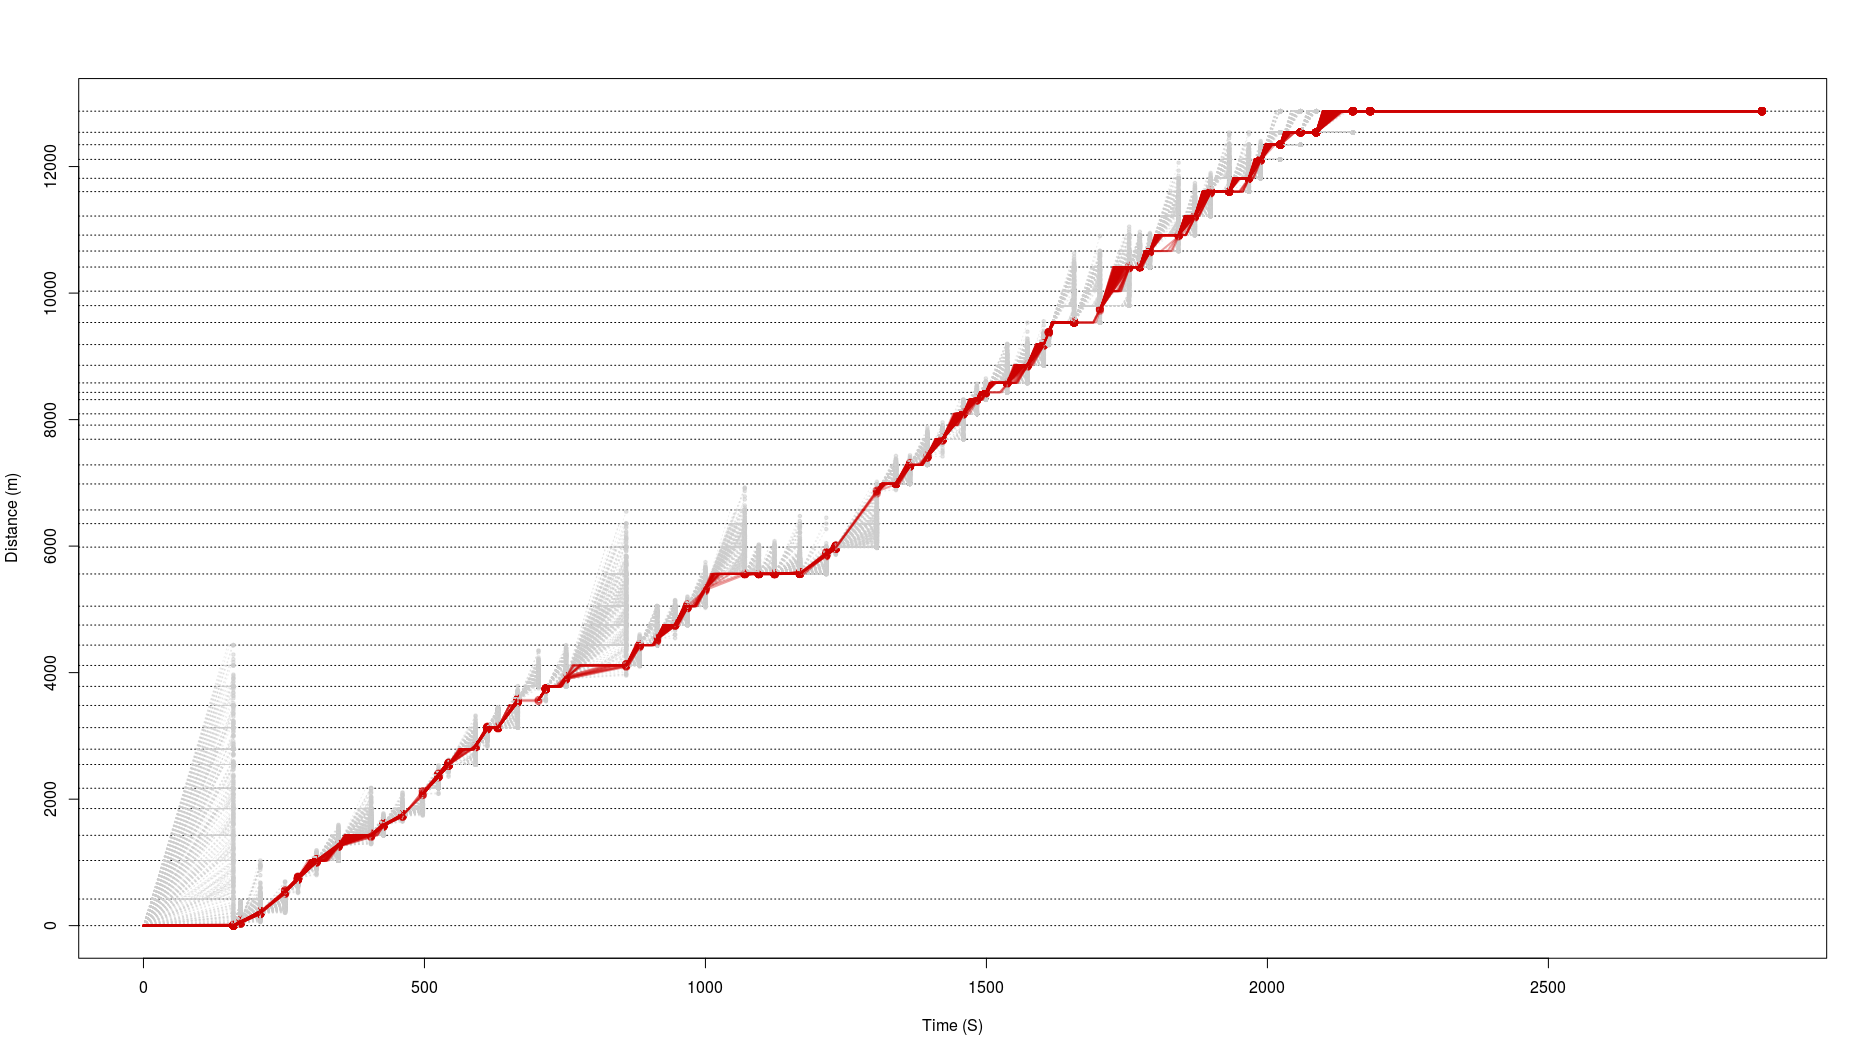
\includegraphics[width=\paperwidth]{figs/complete_route.png}
            };
        \end{tikzpicture}
     \end{frame}
}



\begin{frame}{Arrival Time Prediction}
  \begin{itemize}[<+->]
  \item Use the same ``imaginary buses'' idea

  \item Let each bus (particle) travel and see what time it arrives at future stops

  \item Communicate the distribution of arrival times to commuters:
    \begin{itemize}
    \item Point estimates, e.g., median: ETA 5~minutes
    \item Prediction interval: ETA 4--8~minutes
    \end{itemize}
  \end{itemize}

  \begin{overprint}
    \onslide<1>
    \centering
    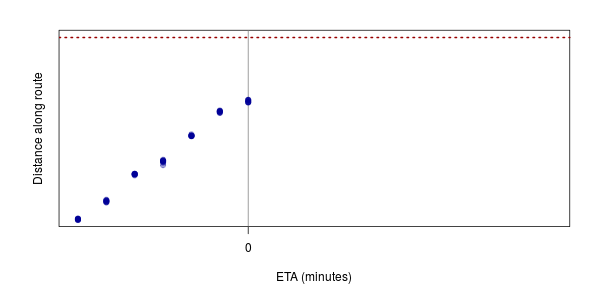
\includegraphics[width=0.8\textwidth]{arrival/particle_arrival1.png}
    \onslide<2-3>
    \centering
    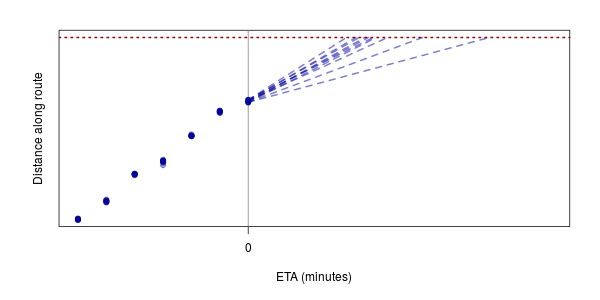
\includegraphics[width=0.8\textwidth]{arrival/particle_arrival2.png}
    \onslide<4>
    \centering
    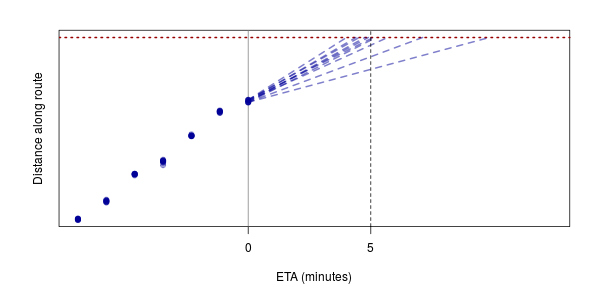
\includegraphics[width=0.8\textwidth]{arrival/particle_arrival3.png}
    \onslide<5>
    \centering
    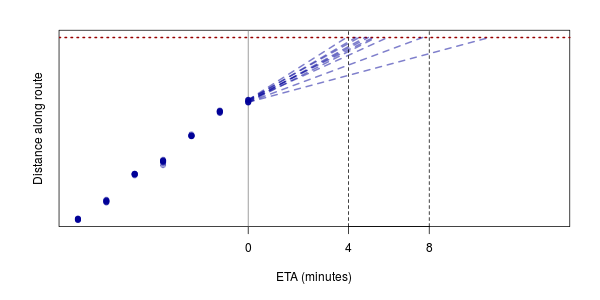
\includegraphics[width=0.8\textwidth]{arrival/particle_arrival4.png}
  \end{overprint}
\end{frame}



% \begin{frame}{Real-time traffic from other buses}
%   \begin{itemize}[<+->]
%   \item Historically, each bus treated independently
%   \item More recently, work on multiple buses sharing a route
%   \item How about buses sharing a road?
%   \end{itemize}
% \end{frame}


\begin{frame}[standout]
  Thank you!
\end{frame}



\end{document}
